\externaldocument{modelling}

\section{Method}\label{sec:method}

This work will investigate how the free parameters of the model given by the equations~\ref{eq:6} -~\ref{eq:10} will affect the spatial temporal progress of the numerical simulation. For the numerical simulation we will use the weak form given with equations~\ref{eq:11} -~\ref{eq:13} and solve it using HiFlow\textsuperscript{3}~\cite{hiflow3}. To study the results of the numerical simulation ParaView~\cite{paraview} is used, producing informative plots to compare the evolution of the simulation in time. For this we rely on the tool Plot Over Line to give results for the three variables of tumour cell density, extracellular matrix density and matrix-degrading enzymes density, an example for this can be seen in figure~\ref{fig:Initial_Value_Distribution} showing the initial conditions. In figure~\ref{fig:PlotOverLine} you can see the configuration for the Plot Over Line tool, since we are consider the experiments on the unit square in 2D dimensional case, the line starts at $x=0.5, y=0.5$ and ends at $x=0.5, y=1$.\newline
\begin{figure}[h]
    \centering
    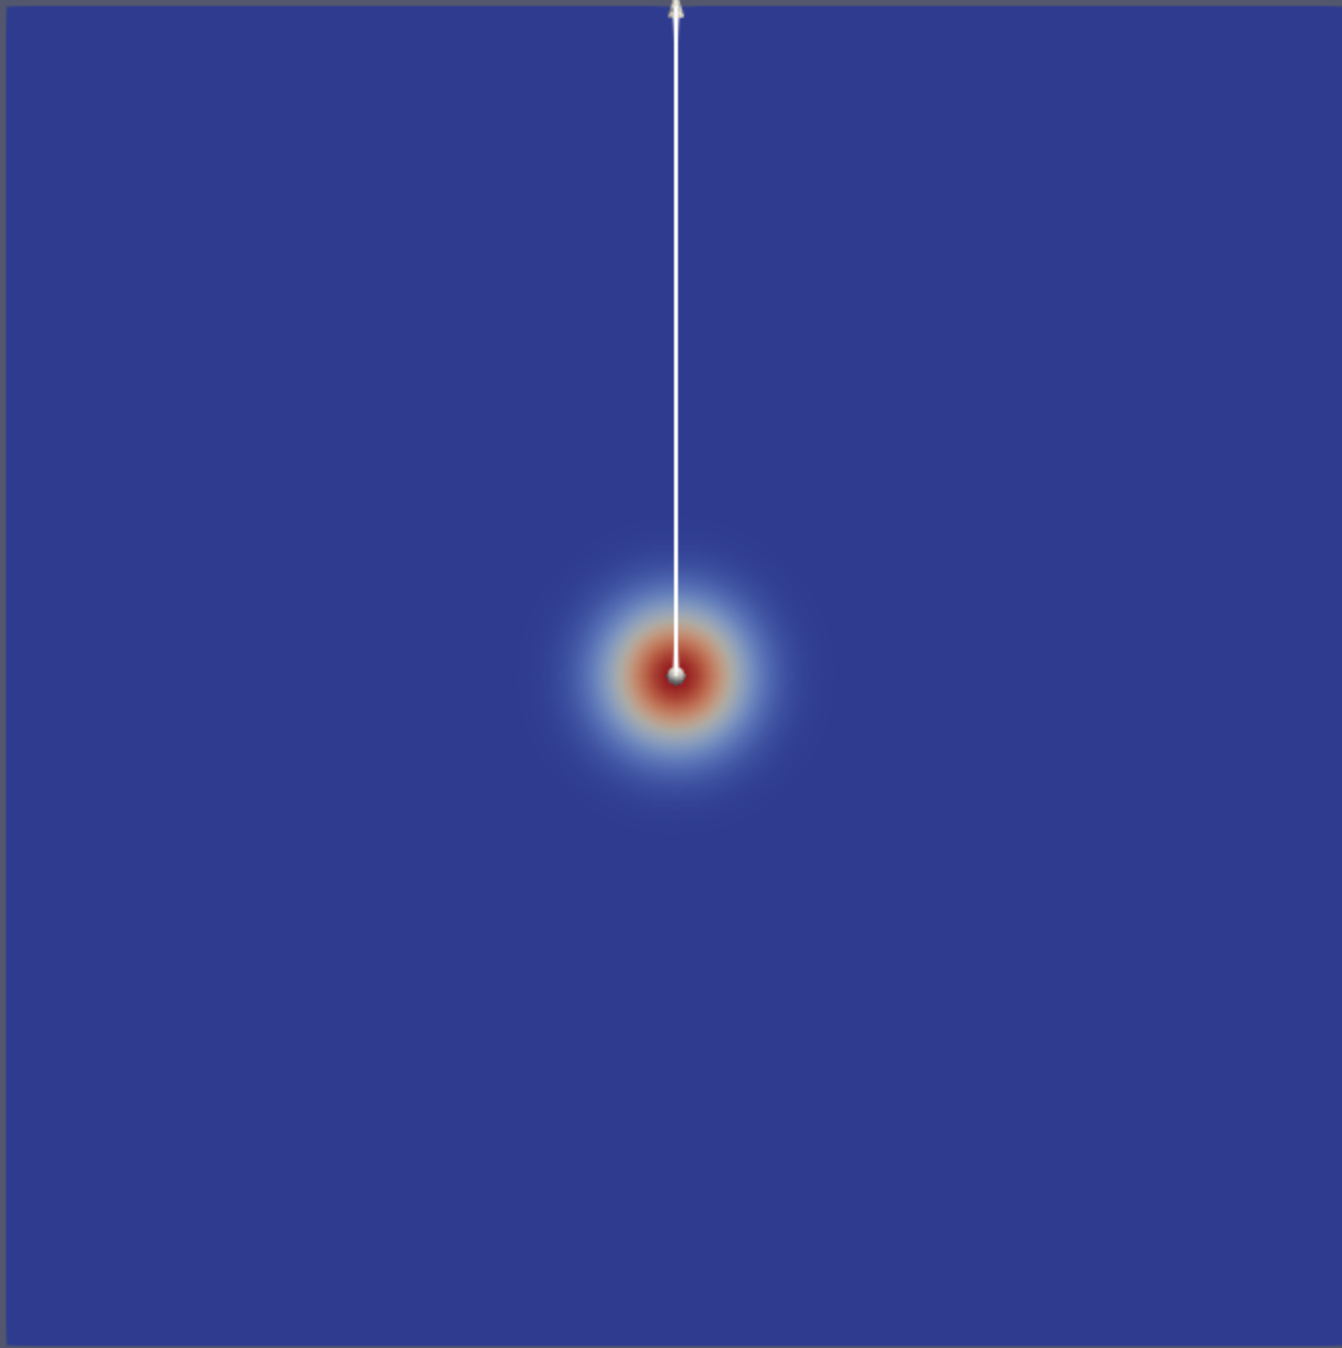
\includegraphics[width=0.3\textwidth]{resources/images/plot_over_line_tool.png}
    \caption{Plot Over Line Tool Configuration}
    \label{fig:PlotOverLine}
\end{figure}

\begin{comment}
All experiments that consider the ECM to be homogenous start with the same initial values as seen in figure~\ref{fig:Initial_Value_Distribution}. Experiments observing the effects of a heterogenous ECM use different initial values, like seen in $\textcolor{red}{initial values heterogenous ECM}$.\newline 
This work starts with \textcolor{red}{trying to replicate/replicating} numerical simulations done by other papers. Since there were only 1D simulations done previously, the model will be adjusted in such a way, that the Plot Over Line graphs mimick the plots given by the previous experiments. This will serve two purposes, first it will verify a correct implementation of the model and second this will give us a starting point by which we can vary the parameters, investigating the phenomena this model exhibits. \newline 
We will start with examining 2D experiments with homogenous ECMs, using our model with the parameters $mu_1$ and $mu_2$ both set to zero, considering a case with no proliferation, after this we will introduce proliferation, varying also $\mu_1$ and $\mu_2$. The same will be done for the 3D cases, also at first neglecting proliferation to apply it in a later stage. Our focus here lies on investigating the effects of the parameters, but also on how the dimension changes results, with fixed free parameters. At last we will have a brief outlook on how a heterogenous ECM influences our results.\newline
The results of the above experiments will be summarized and discussed in the Conclusion and Discussion part, pointing out the important characteristics of the simulations and disucssing the sensitivity of each of the parameters and the influence of the dimension. At this point we will have an outlook on how to extend the model with more continuous and or discrete adaptations. \newline \newline

Looking at the parameter estimates from \cite{anderson_mathematical_2000} to non-dimensionalise the time, we see that with $L \in [0.1cm,1cm]$ and $D\approx 10^{-6}\frac{cm^2}{s}$, $\tau = \frac{L^2}{D}$ gives a relative big temporal range, $\tau_{min} = 1000s = 16.66 min$ and $\tau_{max} = 1000000s = 16666.66min$, which makes it hard, to find the correct time step value to compare our simulation results with the one from \cite{anderson_mathematical_2000} and \cite{Kolev2010}. Another challenge are the diffusion coefficients, since they are dependent on the dimension we are in, we have to find our own estimate as a baseline value. \newline 
For our experiments we will use a set of baseline parameters, which will be evaluated experimentally, and from there vary one parameter at a time to get an overview of their effects and later we will incorporate variation of multiple paramters in accordance with the numerical model. 
\end{comment}

